
\bbsubsection{Adding a New Budget}{add-budget}

The Add New Budget screen enables users to add a new budget by specifying the budget's name and its allotted amount within a specified frequency (that is, Monthly, Weekly, or Daily). The frequency can be selected from the Budget Screen (Section TBA). The user can also add categories within the Budget.

\bbsubsubsection{Application Screenshots}{add-budget-screenshots}

\begin{figure}[h]
 
\begin{subfigure}{0.5\textwidth}
  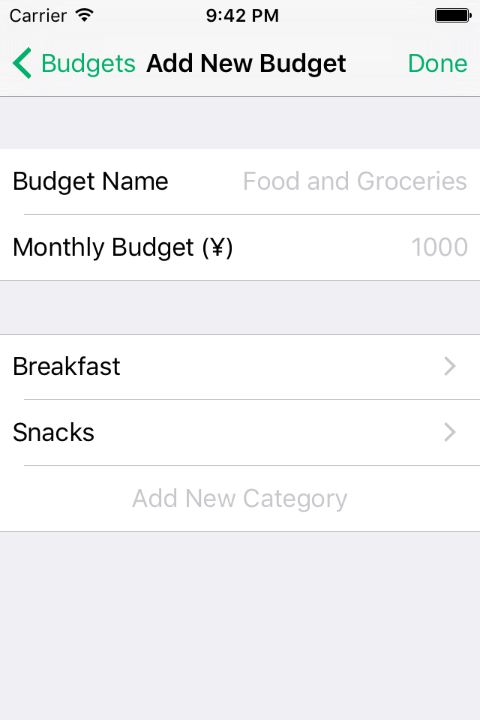
\includegraphics[scale=0.35]{BUD-0001} 
  \caption{Add New Budget Screen}
  \label{fig:sub-budget-1}
\end{subfigure}
\begin{subfigure}{0.5\textwidth}
  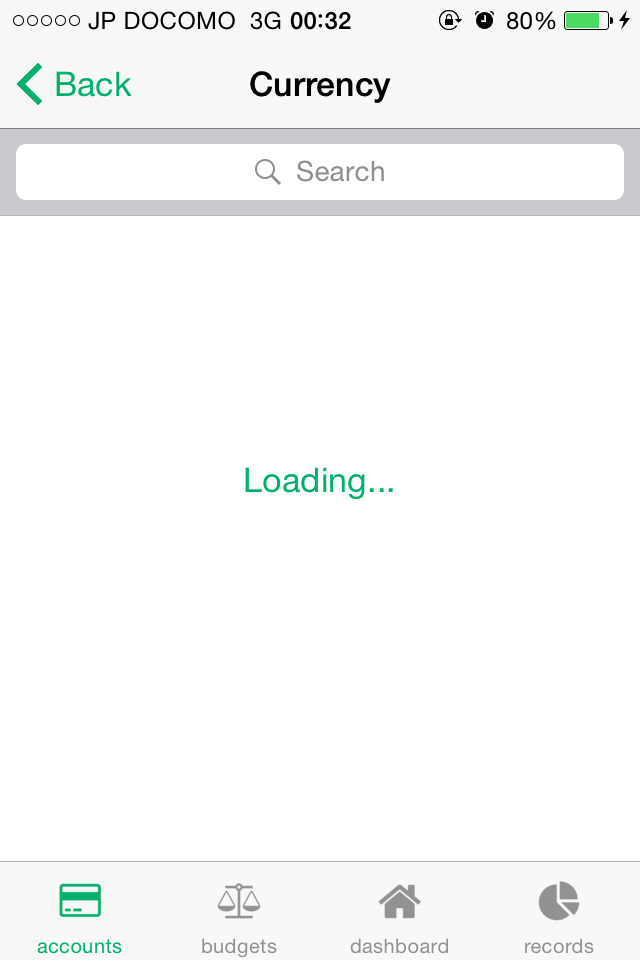
\includegraphics[scale=0.35]{ACC-0001-2}
  \caption{TBD: Edit Category and Swipe to Delete Category}
  \label{fig:sub-budget-2}
\end{subfigure}
\caption{Add New Account Screenshots}
\end{figure}

\screentable{
	\header{Screen Component}
    	{Type}
        {Description}
    \row{1. Screen Title}
    	{Label Title}
        {Localization Key: MENULABEL\_ADD\_BUDGET}
    \row{2. Done Button}
    	{Button}
        {
        When tapped, the app performs form validation and saves all the budget information -- the budget name, and the budget amount -- into the core data. \doublenewline
        For more details on the form validation, please see the \nameref{add-budget-error-scenarios} section. \doublenewline
        Localization Key: BUTTON\_DONE
        } 
    \row{3. Budget Name Cell}
    	{Table Cell}
        {This table cell consists of two UI elements: A label and a textfield. \doublenewline
        
        Tap anywhere in the cell and the textfield will be placed in focus, bringing up a QWERTY keyboard. Tap anywhere outside the cell to dismiss the keyboard. \doublenewline
        
        The textfield has a character limit of 25 characters.\doublenewline
        
        Localization Keys: LABEL\_BUDGET\_NAME, TEXTFIELD\_BUDGET\_PLACEHOLDER} 
    \row{4. Budget Amount Cell}
    	{Table Cell}
        {This table cell consists of two UI elements: A label and a textfield. \doublenewline
        
        Tap anywhere in the cell and the textfield will be placed in focus, bringing up a keyboard that is numeric with a decimal point.  Tap anywhere outside the cell to dismiss the keyboard. \doublenewline

        The label changes in response to what is selected in the Budgets Screen. If the user has chosen "Monthly" in the Budgets Screen, the label will show up as "Monthly Budget", "Weekly Budget" if "Weekly" was chosen, and "Daily Budget" if "Daily" was chosen. (Section X.Y)
        
        The textfield has a character limit of 15 characters.\doublenewline
         
        Localization Keys: LABEL\_MONTHLY, LABEL\_WEEKLY, LABEL\_DAILY, TEXTFIELD\_XLY\_BUDGET\_PLACEHOLDER} 
}

\screentable{
	\header{Screen Component}
    	{Type}
        {Description}
    \row{5. Category Cell}
    	{Table Cell}
        {This table cell consists of a label. \doublenewline
        
        Once the cell is tapped, an alert is brought up, allowing the user to edit the category's name, or delete it.\doublenewline

        The contents of these cells depend on user input in the "Add New Category"
        } 
    \row{6. Add New Category Cell}
    	{Table Cell}
        {This table cell consists of a textfield.\doublenewline
        
        Tap anywhere in the cell and the textfield will be placed in focus, bringing up a QWERTY keyboard. Tap anywhere outside the cell to dismiss the keyboard.\doublenewline
        
        The textfield has a limit of 25 characters.\doublenewline
        
        Localization Keys: LABEL\_IS\_DEFAULT\_ACCOUNT, LABEL\_IS\_DEFAULT\_ACCOUNT\_ DESCRIPTION} 
    \row{7. Error Alert}
    	{Alert Controller}
        {This alert controller has two labels. \doublenewline
        
        The alert is displayed when either the account name or the initial amount has not been filled, and the user taps "Done".\doublenewline
        
        Localization Keys: ERRORLABEL\_ERROR\_TITLE, ERRORLABEL\_NAME\_CURRENCY\_ NOT\_EMPTY}
}

\bbsubsubsection{Error Scenarios}{add-budget-error-scenarios}

\errortable{
	\errorheader{Title}{Description}
    \errorrow{Duplicate Account Name}
    	{This error is triggered when the Done button is pressed and a similar account name already exists in the Core Data. \doublenewline
        
        Localization Key: ERRORLABEL\_ DUPLICATE\_ACCOUNT\_NAME}
    \errorrow{Required Fields Unfilled}
    	{This error is triggered when the Done button is pressed and the account name or the amount has not been filled. \doublenewline
        
        Localization Key: ERRORLABEL\_NAME\_CURRENCY\_ NOT\_EMPTY}
    
    \errorrow{Multiple Decimals}
    	{This check confirms that decimals can only be inputted once. It only exists in textfields that have numeric input. \doublenewline
        
        If a decimal is in the input, and the user keys in another decimal point, the textfield will not respond. There will be no error alert displayed. \doublenewline
        
        If the user pastes text that has two decimal points, then the textfield will not respond as well. Once again, there will be no error alert displayed.
        }
        
    \errorrow{Maximum Length}
    	{This check confirms that the length of the input text is less than or equal to a given number. It is present in all textfields. \doublenewline
        
        Once the maximum length is reached, the user will no longer be able to input any new character. No error alert is displayed.\doublenewline
        
        If the user pastes text that is longer than the maximum length, it will fail to paste and no error alert is displayed.}
}
